\documentclass[11pt]{article}
\usepackage{acl-ijcnlp2009}
\usepackage{times}
\usepackage{url}
\usepackage{latexsym}
%%\newcommand{\review}[1]{{#1}}
\newcommand{\review}[1]{{\textit{Excluded for Review}}}
%\setlength\titlebox{6.5cm}    % You can expand the title box if you
% really have to

\title{\review{KrdWrd} \\
  Architecture for Unified Processing of Web Content}

\author{Johannes Steger\\
  Neurbiopsychology Group\\
  Institute of Cognitive Science\\
  University of Osnabr\"uck\\
  {\tt jsteger@acm.org}  \And
  Egon Stemle\\
  Foo Group\\
  Institute of Cognitive Science\\
  University of Osnabr\"uck\\
  {\tt estemle@uos.de}}

\date{}

\begin{document}
\maketitle
\begin{abstract}

\end{abstract}

\section{Introduction}
Working with algorithms that rely on user-annotated web content suffers from two major deficits:

For annotators, the presentation of web sites in the context of annotation tools usually does not match their everyday web experience.
The lack or degeneration of non-textual context may negatively affect the annotators' performance
and the learning requirements of special annotation tools may make it harder to find and motivate annotators in the first place.

Feature extraction performed on annotated web pages on the other hand leaves much of the information encoded in the page unused,
mainly those concerned with rendering.

In this paper, we present the design (\ref{design}) and implementation (\ref{impl}) of the {\KrdWrd} architecture that addresses these two issues.
Section \ref{casestudy} demonstrates a show-case in the context of the CleanEval challenge and Section \ref{conc} concludes with an outlook on the possible applications and implementation improvements.


\section{Design}
\subsection{Design Goals}

We want to provide an architecture for Web data processing that is based on unified treatment of data on annotation and processing side
and that allows the back-end machinery to access all information contained in a Web page, including how it is presented to a Web surfer.

\subsection{Requirements}

\begin{description}

\item[Flexibility]
The system should be open enough to allow customization of every part, but also specifically provide stable interfaces for more common tasks to allow for modularization.

\item[Stability]
We need a stable HTTP data source that is independent of the original Website, including any dependencies such as images, style-sheets or scripts.

\item[Automaticity]
Back-end processing should run without requiring any kind of human interaction.

\item[Replicability]
Computations carried out on Web pages' representation must be replicable across systems, including any user-side processing.

\item[Quantity]
Corpus size should not influence the performance of the system and total processing time should grow linearly with the corpus.

\item[Usability]
Usability of the annotators side is of paramount importance, so we should stay as close as possible to the everyday Web experience.
We also need to provide tools for learning how to use the annotation tool and how to annotate Web pages.

\end{description}

\subsection{Core Architecture}

To address these requirements, we developed an abstract architecture, a simplified version of which is depicted in figure \ref{f:arch}.
We will outline the rationale for the basic design decisions below.


For rendering a Web page, an object tree is constructed from its HTML source code.
This tree can be traversed and its nodes inspected, modified, deleted and created through an API specified by the World Wide Web Consortium's (W3C) DOM Standard \cite{dom}.
It's most popular use case is client-side dynamic manipulation of Web pages, for visual effects and interactivity.
This is most commonly done by accessing the DOM through a JavaScript interpreter.
Essentially, a page's DOM tree allows access to all the information we set out to work on: structure, textual content and visual rendering data.
We therefore make it the sole interface between application and data.

While all browsers try to implement some part of the DOM standard (currently, version 3 is only partially implemented in most popular browsers), they vary greatly in their level of compliance as well as their ability to cope with non-standard compliant content.
This leads to structural and visual differences between different browsers rendering the same Web page.

Therefore, to guarantee \textit{replicability}, we require the same DOM engine to be used through the system.


To reach a maximal level of \textit{automaticity} and not to limit the \textit{quantity} of the data, it is important that data analysis can take place in a parallel fashion and does not require any kind of graphical interface, so it can e.g. be executed on server farms.
On the other hand we also need to be able to present pages within a browser to allow for user annotation.

Consequently, the same DOM engine needs to power a browser as well as a headless back-end application, with \textit{usability} being an important factor in the choice of a particular browser.


The annotation process, especially the order of presentation of pages, is controlled by a central Web server.
Thereby any number of concurrent annotators can be coordinated and submissions distributed equally across corpora.
All data, un-classified and user-submitted, is stored in a database attached to the Web server.
This setup allows the architecture to scale \textit{automatically} with user numbers under any usage pattern and submission \textit{quantity}.


\textit{Stability} of data sources is a major problem when dealing with Web data.
As we work on Web pages and the elements contained in them, simple HTML dumping is not an option.
Instead, we use a HTTP proxy to cache Web data used in our own storage.
By setting the server to grab content only upon first request and providing a option to turn off download of new data, we can create a closed system that does not change anymore once populated.


\begin{figure}
\jss{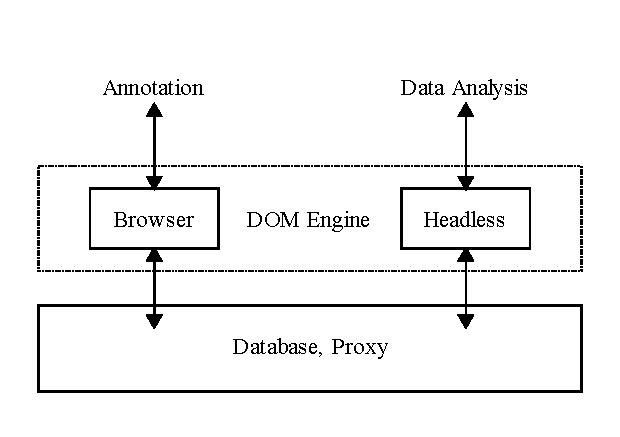
\includegraphics[width=0.4\textwidth]{arch}}
	{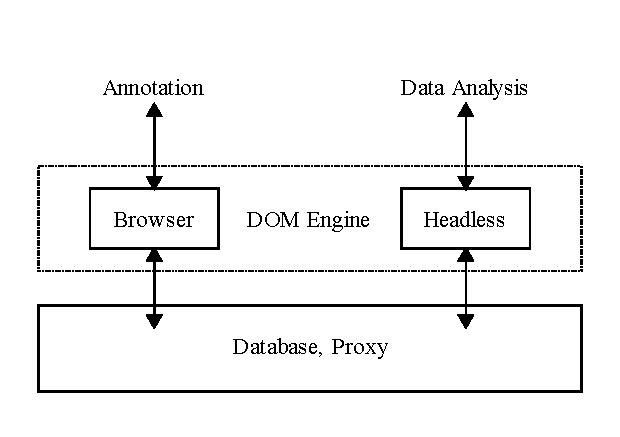
\includegraphics[width=0.8\textwidth]{arch}}
\caption{\label{f:arch}Basic {\KrdWrd} architecture: both users annotating corpus pages through their Web browser
and back-end applications working on the data run the same DOM engine.
	The central server delivers and stores annotation data and coordinates user submissions.}
\end{figure}




\section{Implementation}
\subsection{DOM Engine}

KHTML/WebKit (KDE, Apple), JavaScriptCore or V8 (Google);
The Gecko engine (Mozilla Corporation) and it's JavaScript implementation Spidermonkey;
We briefly checked on Presto (Opera) and Trident (Microsoft), but discarded them due to their proprietary nature.

\subsubsection{Firefox AddOn}

To avoid interference with other AddOns and existing configuration, we suggest creating a new browser profile for use with the AddOn.
For easy use, Firefox' proxy configuration is automatically pointed to a preconfigured host and the user is directed to a special landing page upon successful installation.
visual tagging, results

\begin{figure}
\jss{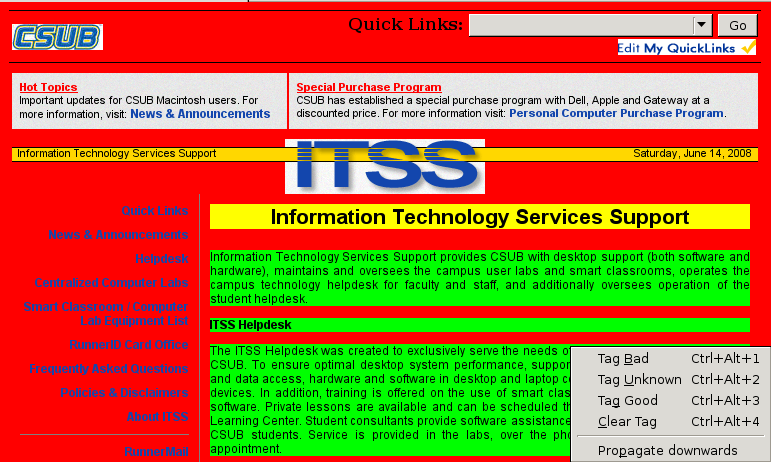
\includegraphics[width=0.5\textwidth]{tut0}}
	{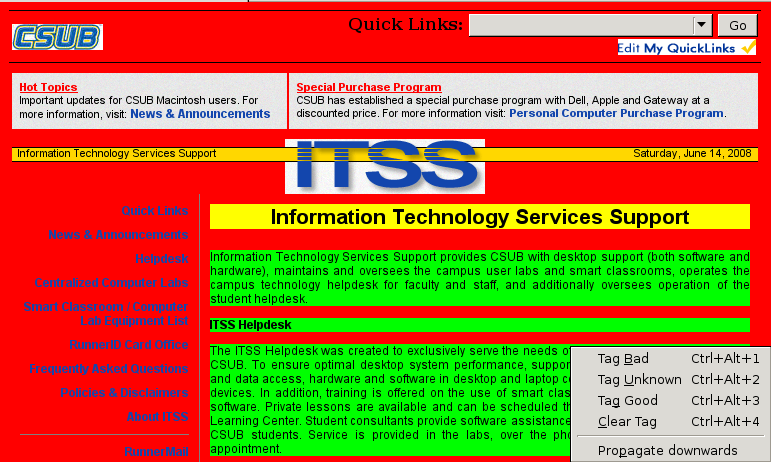
\includegraphics[width=\textwidth]{tut0}}
\caption{\label{f:tut0}Web pages can be annotated with the KrdWrd Firefox AddOn by hovering over the text by mouse and setting class labels by keyboard shortcut or pop-up menu}
\end{figure}


\subsubsection{XUL Application}

The XUL application (or \textit{app} for short) 
Dumper, Grabber, Crawler

% ens said: if you like:
% \cite{NajorkHeydon2001,ShkapenyukSuel2002}

\subsection{Storage and Control}

database and web server. 

\subsubsection{Web Server}

small Python CGI scripts;
provides per-corpora submission list,
controls serving of random corpus pages;
tutorial mode: visual diff after submit;
ssl connections only;

\begin{figure}
\jss{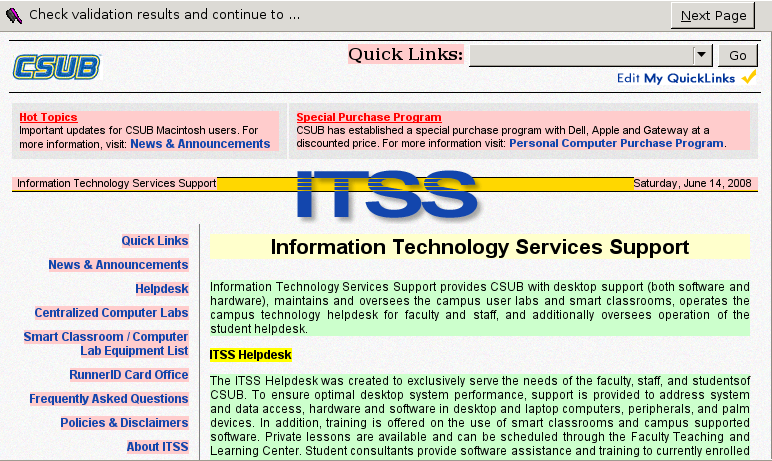
\includegraphics[width=0.5\textwidth]{tut1}}
	{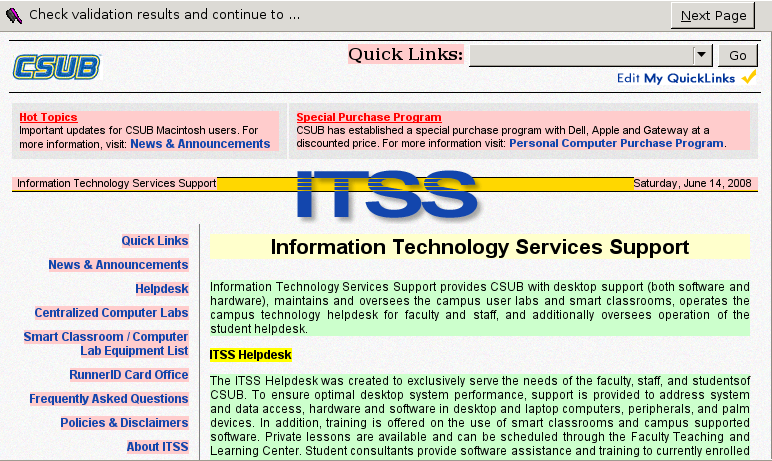
\includegraphics[width=\textwidth]{tut1}}
\caption{\label{f:tut1}During the tutorial, a Visual Diff between the user's submission and the sample data is presented right after submission.
	Here, the annotation from \ref{f:tut0} was wrong in tagging the sub-heading ``ITSS Helpdesk'': the correct annotation (\textit{yellow}) is highlighted in the feedback.}
\end{figure}

\subsubsection{Database}

Raw HTML in sqlite3;
user submissions are anonymized, but trackable by id;

\subsubsection{Proxy}

\begin{figure}
\jss{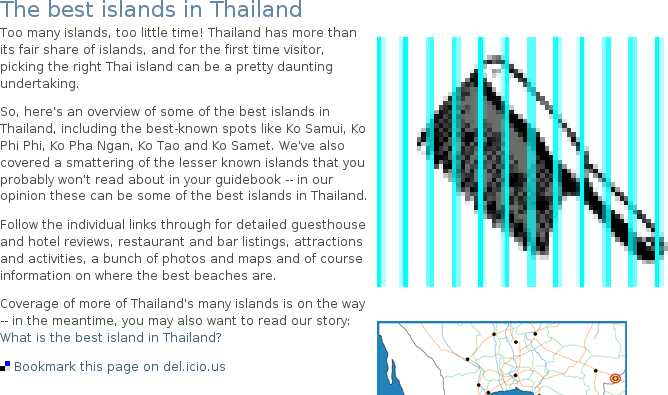
\includegraphics[width=0.5\textwidth]{add}}
	{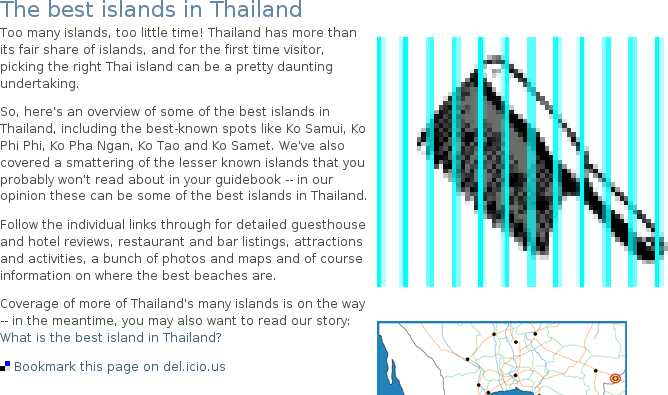
\includegraphics[width=\textwidth]{add}}
\caption{IFrames with dynamic URLs which usually come from advertisements are blocked as a nice side-effect of the Proxy setup}
\end{figure}

\subsection{Feature Extractors}

app produces input files for pipelines, dumped in the filesystem, per-page with one line per dom text node;
integrated dom feature extraction;
integrated screen grab;

\subsubsection{Text}

Dumped raw text, leading and trailing whitespace removed, UTF-8.

\subsubsection{Meta Visual}

Use data from living DOM Tree in XUL App.

\subsubsection{Visual}

Screenshot and use JAMF as seen in \cite{Steger08}
\footnote{This Extractor requires at least XULRunner Version 1.9.2 (corresponding to Firefox Version 3.5) which is still in beta at the time of this writing}

\subsection{Machine Learner}

Generic input vectors and classes from extractors

\subsection{\label{sec:limitations}Highlights and Limitations}

html, utf, js, iframes


\section{Use Cases}

\subsection{Cleaneval}
\subsubsection{Data Acquisition}
crawling simple

students: fast, no probs with tool

\subsubsection{Extraction Pipeline}

\subsubsection{Results}

\subsection{Future Work}
can cure cancer.

\section{Conclusion}
introduced, shown to work, now you get started.

\review{
\section*{Acknowledgments}

}

\bibliographystyle{acl}
\bibliography{bib}

\end{document}
